\documentclass[]{article}
\usepackage[T1]{fontenc}
\usepackage{lmodern}
\usepackage{amssymb,amsmath}
\usepackage{ifxetex}
\usepackage{fixltx2e} % provides \textsubscript
% use microtype if available
\IfFileExists{microtype.sty}{\usepackage{microtype}}{}
\ifnum 0\ifxetex 1\fi=0 % if pdftex
  \usepackage[utf8]{inputenc}
\else % if xelatex
  \usepackage{fontspec}
  \ifxetex
    \usepackage{xltxtra,xunicode}
  \fi
  \defaultfontfeatures{Mapping=tex-text,Scale=MatchLowercase}
  \newcommand{\euro}{€}
\fi
\usepackage{color}
\usepackage{fancyvrb}
\DefineShortVerb[commandchars=\\\{\}]{\|}
\DefineVerbatimEnvironment{Highlighting}{Verbatim}{commandchars=\\\{\}}
% Add ',fontsize=\small' for more characters per line
\newenvironment{Shaded}{}{}
\newcommand{\KeywordTok}[1]{\textcolor[rgb]{0.00,0.44,0.13}{\textbf{{#1}}}}
\newcommand{\DataTypeTok}[1]{\textcolor[rgb]{0.56,0.13,0.00}{{#1}}}
\newcommand{\DecValTok}[1]{\textcolor[rgb]{0.25,0.63,0.44}{{#1}}}
\newcommand{\BaseNTok}[1]{\textcolor[rgb]{0.25,0.63,0.44}{{#1}}}
\newcommand{\FloatTok}[1]{\textcolor[rgb]{0.25,0.63,0.44}{{#1}}}
\newcommand{\CharTok}[1]{\textcolor[rgb]{0.25,0.44,0.63}{{#1}}}
\newcommand{\StringTok}[1]{\textcolor[rgb]{0.25,0.44,0.63}{{#1}}}
\newcommand{\CommentTok}[1]{\textcolor[rgb]{0.38,0.63,0.69}{\textit{{#1}}}}
\newcommand{\OtherTok}[1]{\textcolor[rgb]{0.00,0.44,0.13}{{#1}}}
\newcommand{\AlertTok}[1]{\textcolor[rgb]{1.00,0.00,0.00}{\textbf{{#1}}}}
\newcommand{\FunctionTok}[1]{\textcolor[rgb]{0.02,0.16,0.49}{{#1}}}
\newcommand{\RegionMarkerTok}[1]{{#1}}
\newcommand{\ErrorTok}[1]{\textcolor[rgb]{1.00,0.00,0.00}{\textbf{{#1}}}}
\newcommand{\NormalTok}[1]{{#1}}
\usepackage{graphicx}
% We will generate all images so they have a width \maxwidth. This means
% that they will get their normal width if they fit onto the page, but
% are scaled down if they would overflow the margins.
\makeatletter
\def\maxwidth{\ifdim\Gin@nat@width>\linewidth\linewidth
\else\Gin@nat@width\fi}
\makeatother
\let\Oldincludegraphics\includegraphics
\renewcommand{\includegraphics}[1]{\Oldincludegraphics[width=10cm]{#1}}
\ifxetex
  \usepackage[setpagesize=false, % page size defined by xetex
              unicode=false, % unicode breaks when used with xetex
              xetex]{hyperref}
\else
  \usepackage[unicode=true]{hyperref}
\fi
\hypersetup{breaklinks=true,
            bookmarks=true,
            pdfauthor={},
            pdftitle={},
            colorlinks=true,
            urlcolor=blue,
\usepackage[margin=1.8cm]{geometry}
\author{
Lovelace, Robin\\
\texttt{r.lovelace@leeds.ac.uk}
}
\title{Open Street Map: loading, analysing and visualising free maps with R and QGIS}
            linkcolor=magenta,
            pdfborder={0 0 0}}
\maketitle
\setlength{\parindent}{0pt}
\setlength{\parskip}{6pt plus 2pt minus 1pt}
\setlength{\emergencystretch}{3em}  % prevent overfull lines
\setcounter{secnumdepth}{0}

\author{}
\date{}

\begin{document}




This tutorial shows how open source tools can be used to harness a huge
and rapidly growing open source geodatabase: Open Street Map. It is
targeted at people new to Open Street Map, but who already have an
understanding of basic GIS concepts. Previous experience with the
programs QGIS and R would be beneficial, but not essential, for
completing the excercises. There are also a number of resources
available on-line for more advanced functions, as described below.

\section{Introduction}

Open Street Map (OSM) is a crowd-sourced map of the world, the archetype
of `volunteered geographical information'
(\href{http://www.ncgia.ucsb.edu/projects/vgi/docs/position/Goodchild\_VGI2007.pdf}{Goodchild
2007}). The aim is simple: ``to create a set of map data that's free to
use, editable, and licensed under new copyright schemes'', as described
in an excellent review article on the subject
(\href{http://discovery.ucl.ac.uk/13849/1/13849.pdf}{Haklay and Weber
2008}). Putting the public in charge of editing the world's surface may
seem like a risky business, given that cartographers have specialist
skills developed over centuries. This issue is described in
\href{https://dl.dropboxusercontent.com/u/15008199/egs2stay/Mapping\_the\_Void\_-\_Mapping\_the\_Void\_b03s6mf0\_default.m4a}{Mapping
the Void}, an excellent BBC Radio 4 Documentary on the subject
(Salisbury and Jenkins 2014). Yet the emergence of high resolution
aerial photography covering the entirety of the Earth's surface and the
explosion in GPS ownership via smartphones has enabled citizens to
become accurate sensors of the world.
\href{http://www.mdpi.com/1999-5903/4/1/1/pdf}{Neis et al. (2012)}
believe this phenomenon is more than merely technological. In OSM, they
see a ``revolutionary paradigm shift on how map data is being
collected''. Citizen mappers have the added advantage that they may know
their local area far better than any professional cartographer.

This tutorial adds a small nugget of information to the growing
literature on OSM, by demonstrating how the data can be accessed for
teaching or research materials. It's a completely free and open dataset,
so we may as well use it! There is already some good on-line material
about OSM data, including:

\begin{itemize}
\item
  a \href{http://www.mdpi.com/1999-5903/5/2/282/pdf}{paper} comparing
  the quality and coverage of OSM map data in different parts of the
  world
\item
  an
  \href{http://www.library.carleton.ca/sites/default/files/help/gis/WorkingWithOpenStreetMap.pdf}{overview}
  of handling OSM data in ArcMap
\item
  a
  \href{http://elogeo.nottingham.ac.uk/xmlui/bitstream/handle/url/289/osm-tutorial-final-2.pdf?sequence=1}{tutorial}
  illustrating its potential use for GIS education and store location
  planning
\end{itemize}

Yet nothing has focussed on simply loading the data using different
tools. In this paper we use QGIS and R because these are (arguably) the
most popular open source programmes used by geographers, the discipline
with most to gain from OSM data. Before delving into the method (which
is actually quite straightforward), let's put OSM data in context.

\subsection{Why (and why not) use OSM data?}

Of course there are teething issues with any large-scale open source
database, including variable data quality, patchy and incomplete
coverage and inconsistencies from place to place (Haklay 2010). Yet all
of these issues are gradually being ironed out. The advantages of Open
Street Map outweigh these downsides for many applications
\emph{already}. These include:

\begin{itemize}
\item
  Rapid updates of new projects
\item
  Greater range of attributes (e.g.~shop names)
\item
  Ability to share data with anyone without breaching license
\end{itemize}

In additions there are a number of ethical benefits of using OSM: it's
community a map for the greater good
(\href{http://www.theguardian.com/technology/2014/jan/14/why-the-world-needs-openstreetmap}{Wroclawski
2014}).

There is a strong community of OSM volunteers who use the service for
humanitarian purposes (Salisbury and Jenkins 2014). Two excellent
examples of this help underline the ethical side of OSM data.
\href{http://explore.ramanitanzania.org/}{Tindale}, a settlement in
Tanzania that has been mapped rapidly thanks to a single academic
project, in collaboration with the authorities, enabling better policy
making in the area (see
\href{http://www.youtube.com/watch?v=KqrGyvNnWkA}{video}). Second, the
rapid response of the OSM community to the Typhoon Haiyan disaster. In a
matter of days, an army of volunteers had helped to map out the affected
zone, aiding relief efforts (e.g.~see
\href{https://www.mapbox.com/blog/typhoon-haiyan-openstreetmap/}{MapBox's
blog posts on the subject}).

\subsection{An overview of the tutorial}

All of the code and data used to create this tutorial is available on
\href{http://github.com}{GitHub}. Feel free to download the project as a
\texttt{.zip} file from the
\href{https://github.com/Robinlovelace/osm-tutorial}{project's
repository} entitled osm-tutorial from github.com/Robinlovelace. This
zip file contains all of the code and data used to generate the
tutorial, which is entirely reproducible. If you would like to modify or
improve it in any way, please fork a version for you own use, citing the
original where appropriate.

The focus is mainly on the technical challenge of extracting the data
from servers `in the cloud' and onto your desktop. We also cover some
basic tasks in handling, subsetting and visualising the data, first in
the graphical user interface (GUI) of QGIS, and then in the command line
with R. The next stage talks about editing raw OSM data, essential if
you would like to take subsets of very large OSM datasets, such as
\texttt{planet.osm} which takes up more than 30 GB of memory. The next
stage is to talk about OSM data in PostGIS, a geodatabase program ideal
for querying very large spatial datasets. Finally, there is a brief
section on further resources. None of the sections require any of the
previous ones although the level of difficulty generally increases as
you progress.

\section{Getting the data}

OSM data of a specific area can be downloaded directly from the
\href{http://www.openstreetmap.org}{main map page}, from the
\href{http://overpass-api.de/}{Overpass API} or, for the entire planet,
from the huge (currently 32 GB)
\href{http://planet.openstreetmap.org/}{planet.osm file}. A number of
third parties also provide more manageable chunks of this dataset, such
as the single country datasets provided by
\href{http://download.geofabrik.de/}{GEOFABIK}. Command line programs
\href{http://wiki.openstreetmap.org/wiki/Osmosis}{Osmosis} and
\href{http://wiki.openstreetmap.org/wiki/Osm2pgsql}{Osm2pgsl} can be
used to process raw OSM data in either \texttt{.osm} or
\texttt{.osm.pbf} file formats. The former is essentially a
\texttt{.xml} (Extensible Markup Language) text file (encoded with the
popular UTF-8 characterset); the latter is a compressed version of the
former. How we transfer these datasets into a useful form depends on the
program you are using. In this tutorial we will explain how to do it in
QGIS and R, as well describing the basics of getting it into a
\href{http://postgis.net/}{PostGIS} database.

\section{OSM data in QGIS}

A \texttt{.osm} file can be downloaded from the openstreetmap.org with
the bounding box selected by default depending on the current view, or
via a manual selection, as shown below.

\begin{figure}[htbp]
\centering
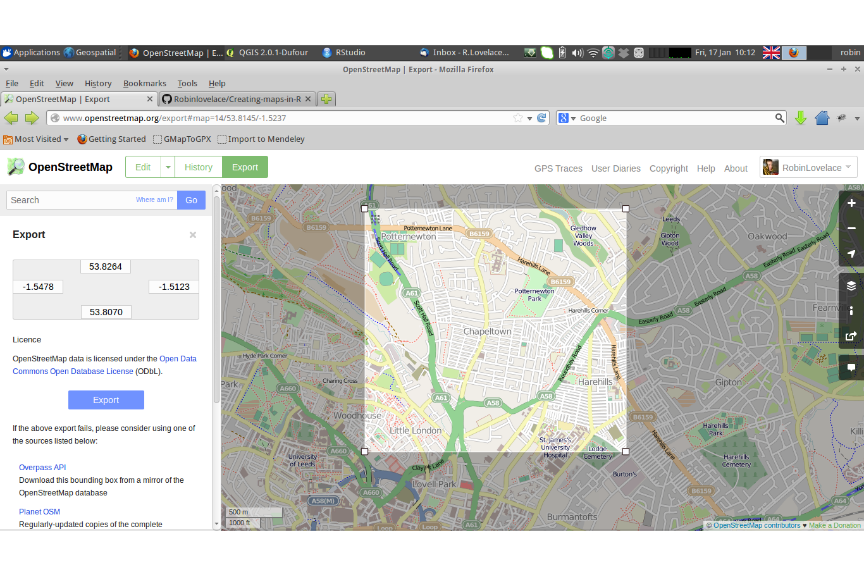
\includegraphics{figure/Manual_selection_of_bounding_box.png}
\caption{Manual selection of bounding box}
\end{figure}

To load this file into QGIS, you can simply use the
\texttt{Add Vector Layer} button on the left of the screen. However this
does not generate satisfactory results. The \emph{recommended} way to
import the data is via the the OSM plugin. When this is installed in
QGIS 2.0, use the menus \texttt{Vector \textgreater{} OpenStreetMap} to
import the xml file and convert it into a SpatiaLite database. Then you
can import it into the QGIS workspace.

\begin{figure}[htbp]
\centering
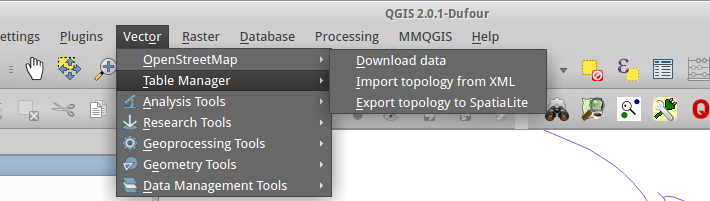
\includegraphics{osmfigs/import-osm.png}
\caption{Import the osm data to SpatiaLite}
\end{figure}

After this step the file has been saved as a \texttt{.osm.db} file. Use
the \texttt{Export Topology to SpatiaLite} element of the same menu to
load the file. Choose the type of spatial data you would like to load -
Points, Lines or Polygons. At this stage one can also select which
variables (``Tags'') you would like to add to the attribute data.

\begin{figure}[htbp]
\centering
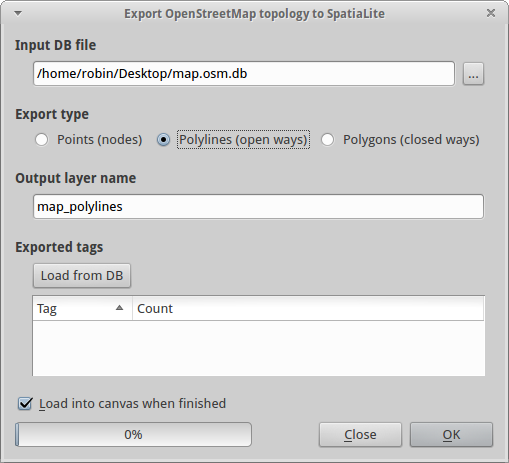
\includegraphics{osmfigs/open-osmdb.png}
\caption{Select Polylines}
\end{figure}

The data is now loaded into QGIS allowing standard methods of analysis.
You will notice that the data are not styled at all, leading to very
bland maps. To counter this, there have been custom styles developed for
visualising OSM data in QGIS, e.g.
\href{http://anitagraser.com/2012/02/25/light-styles-for-osm-layers-in-qgis/}{those
by Anita Grazer}. Unfortunately these files do not seem to be working
with the current version of QGIS so alternative ready-made styles must
be created, as suggested by a
\href{http://gis.stackexchange.com/questions/42645/is-there-up-to-date-osm-sld-file-for-geoserver}{stackexchange
question}.

Once the data is loaded into QGIS, it can be used as with any other
spatial data. Next, let's see how R can handle OSM data, via the
\texttt{osmar} package.

\section{Using osmar}

\texttt{osmar} is an R package for downloading and interrogating OSM
data that accesses the data directly from the internet via the R command
line. There is an excellent
\href{http://journal.r-project.org/archive/2013-1/eugster-schlesinger.pdf}{online
tutorial} which provides a detailed account of the package (Eugster \&
Schlesinger, 2012). Here we will focus on loading some basic data on
bicycle paths in Leeds. First the package must be loaded:

\begin{Shaded}
\begin{Highlighting}[]
\KeywordTok{library}\NormalTok{(osmar)  }\CommentTok{# if the package is not already installed, use install.packages('osmar')}
\end{Highlighting}
\end{Shaded}

\begin{verbatim}
## Loading required package: XML
## Loading required package: RCurl
## Loading required package: bitops
## Loading required package: geosphere
## Loading required package: sp
## 
## Attaching package: 'osmar'
## 
## The following object is masked from 'package:utils':
## 
##     find
\end{verbatim}

To download data directly, one first sets the source and a bounding box,
and then use the \texttt{get\_osm} function to download it. Selecting
Chapeltown as the centrepoint of the map, we can download all the data
in the square km surrounding it.

\begin{Shaded}
\begin{Highlighting}[]
\NormalTok{src <- }\KeywordTok{osmsource_api}\NormalTok{()}
\NormalTok{bb <- }\KeywordTok{center_bbox}\NormalTok{(-}\FloatTok{1.53492}\NormalTok{, }\FloatTok{53.81934}\NormalTok{, }\DecValTok{1000}\NormalTok{, }\DecValTok{1000}\NormalTok{)}
\NormalTok{ctown <- }\KeywordTok{get_osm}\NormalTok{(bb, }\DataTypeTok{source =} \NormalTok{src)}
\KeywordTok{plot}\NormalTok{(ctown)}
\KeywordTok{points}\NormalTok{(-}\FloatTok{1.53492}\NormalTok{, }\FloatTok{53.81934}\NormalTok{, }\DataTypeTok{col =} \StringTok{"red"}\NormalTok{, }\DataTypeTok{lwd =} \DecValTok{5}\NormalTok{)}
\end{Highlighting}
\end{Shaded}

\begin{figure}[htbp]
\centering
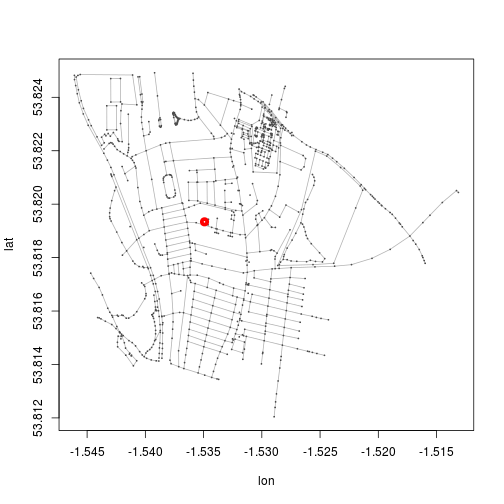
\includegraphics{figure/Preliminary_plot_of_Chapletown_with_osmar.png}
\caption{Preliminary plot of Chapletown with osmar}
\end{figure}

This shows that the data has successfully been loaded and saved as an
object called \texttt{ctown}. Let's try analysing this object further.
In fact, \texttt{ctown} is technically a list, composed of 3 objects:
nodes (points), ways (lines) and relations (polygons composed of many
lines). Such OSM data is thus provided a class of its own, and each
sub-object can be called separately using the \texttt{\$} symbol:

\begin{Shaded}
\begin{Highlighting}[]
\KeywordTok{names}\NormalTok{(ctown)}
\end{Highlighting}
\end{Shaded}

\begin{verbatim}
## [1] "nodes"     "ways"      "relations"
\end{verbatim}

\begin{Shaded}
\begin{Highlighting}[]
\KeywordTok{class}\NormalTok{(ctown)}
\end{Highlighting}
\end{Shaded}

\begin{verbatim}
## [1] "osmar" "list"
\end{verbatim}

\begin{Shaded}
\begin{Highlighting}[]
\KeywordTok{summary}\NormalTok{(ctown$ways)}
\end{Highlighting}
\end{Shaded}

\begin{verbatim}
## osmar$ways object
## 179 ways, 505 tags, 1270 refs 
## 
## ..$attrs data.frame: 
##     id, visible, timestamp, version, changeset, user, uid 
## ..$tags data.frame: 
##     id, k, v 
## ..$refs data.frame: 
##     id, ref 
##  
## Key-Value contingency table:
##            Key               Value Freq
## 1      highway         residential   71
## 2  source:name OS_OpenData_Locator   49
## 3      highway             service   41
## 4   created_by                JOSM   25
## 5       source                Bing   23
## 6      highway        unclassified   17
## 7      highway             footway   15
## 8     building                 yes   11
## 9          lit                 yes   11
## 10      source                 npe   10
\end{verbatim}

Let's use the dataset we have loaded to investigate the cycle paths in
the vicinity of my house. First we need to understand the data contained
in the object. Let's look at the tags and the attributes of the
\texttt{ways} object:

\begin{Shaded}
\begin{Highlighting}[]
\KeywordTok{summary}\NormalTok{(ctown$ways$tags)  }\CommentTok{# summary of the tag data}
\end{Highlighting}
\end{Shaded}

\begin{verbatim}
##        id                     k                         v      
##  Min.   :5.09e+06   highway    :155   residential        : 71  
##  1st Qu.:7.73e+06   name       :128   OS_OpenData_Locator: 49  
##  Median :8.46e+07   source     : 56   service            : 41  
##  Mean   :8.71e+07   source:name: 54   yes                : 32  
##  3rd Qu.:1.50e+08   created_by : 25   JOSM               : 25  
##  Max.   :2.45e+08   building   : 12   Bing               : 23  
##                     (Other)    : 75   (Other)            :264
\end{verbatim}

\begin{Shaded}
\begin{Highlighting}[]
\KeywordTok{head}\NormalTok{(ctown$ways$attrs, }\DecValTok{8}\NormalTok{)  }\CommentTok{# attributes of first 8 ways - see I'm in there!}
\end{Highlighting}
\end{Shaded}

\begin{verbatim}
##         id visible           timestamp version changeset            user
## 1  5088536    true 2013-02-22 22:08:24      13  15128484 CompactDstrxion
## 2 22818969    true 2012-09-08 23:06:53      20  13039300    LeedsTracker
## 3  6273628    true 2007-09-21 17:25:37       1    483846          SteveC
## 4  6273619    true 2012-12-01 17:57:45       2  14114856            sc71
## 5  6273721    true 2007-09-16 17:23:14       1    444107            noii
## 6  6273722    true 2007-09-16 17:23:16       1    444107            noii
## 7  6273726    true 2007-09-16 17:23:20       1    444107            noii
## 8  6273736    true 2013-11-02 10:56:24       5  18672988   RobinLovelace
##      uid
## 1 464727
## 2   2330
## 3    682
## 4 106831
## 5  13550
## 6  13550
## 7  13550
## 8 231314
\end{verbatim}

From looking at the \href{http://wiki.openstreetmap.org/wiki/Tags}{OSM
tagging system}, we can deduce that \texttt{id} is the element's id,
\texttt{k} refers to the OSM key (the variables for which the element
has values) and that \texttt{v} is the value assigned for each id - key
combination. Because OSM data is not a simple data frame, we cannot use
the usual R notation for subsetting. Instead we use the \texttt{find}
function. Let us take a subset of bicycle paths in the area and plot
them.

\begin{Shaded}
\begin{Highlighting}[]
\NormalTok{bikePaths <- }\KeywordTok{find}\NormalTok{(ctown, }\KeywordTok{way}\NormalTok{(}\KeywordTok{tags}\NormalTok{(k == }\StringTok{"bicycle"} \NormalTok{& v == }\StringTok{"yes"}\NormalTok{)))}
\NormalTok{bikePaths <- }\KeywordTok{find_down}\NormalTok{(ctown, }\KeywordTok{way}\NormalTok{(bikePaths))}
\NormalTok{bikePaths <- }\KeywordTok{subset}\NormalTok{(ctown, }\DataTypeTok{ids =} \NormalTok{bikePaths)}
\KeywordTok{plot}\NormalTok{(ctown)}
\KeywordTok{plot_ways}\NormalTok{(bikePaths, }\DataTypeTok{add =} \NormalTok{T, }\DataTypeTok{col =} \StringTok{"red"}\NormalTok{, }\DataTypeTok{lwd =} \DecValTok{3}\NormalTok{)}
\end{Highlighting}
\end{Shaded}

\begin{figure}[htbp]
\centering
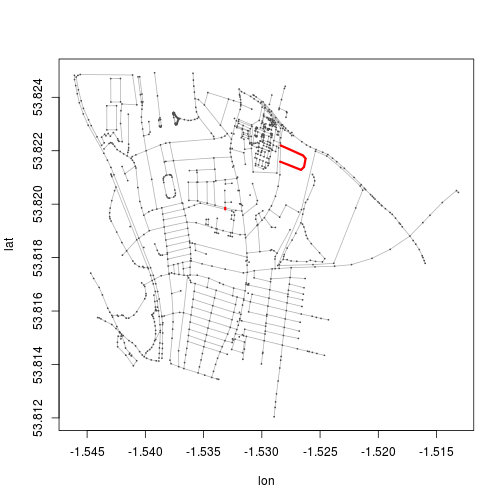
\includegraphics{figure/Bike_paths_of_Chapeltown.png}
\caption{Bike paths of Chapeltown}
\end{figure}

The above code block is used to identify all ways in which cycling is
permitted, ``overriding default access'', according OSM's excellent
\href{http://wiki.openstreetmap.org/wiki/Bicycle}{wiki page on bicycle
paths}.

According to this source, the correct way to refer to an on-road cycle
path is with the \texttt{cycleway} tag. However, none of these have been
added to the roads that have on-road cycle lanes in this example dataset
(as of January 2014). Perhaps someone will add these soon.

\begin{Shaded}
\begin{Highlighting}[]
\KeywordTok{which}\NormalTok{(ctown$ways$tags$k == }\StringTok{"cycleway"}\NormalTok{)}
\end{Highlighting}
\end{Shaded}

\begin{verbatim}
## integer(0)
\end{verbatim}

There are, by contrast, a large number of ways classified as
``residential''. Let us use the same method to select them and add them
to the map.

\begin{Shaded}
\begin{Highlighting}[]
\NormalTok{res <- }\KeywordTok{find}\NormalTok{(ctown, }\KeywordTok{way}\NormalTok{(}\KeywordTok{tags}\NormalTok{(k == }\StringTok{"highway"} \NormalTok{& v == }\StringTok{"residential"}\NormalTok{)))}
\NormalTok{res <- }\KeywordTok{find_down}\NormalTok{(ctown, }\KeywordTok{way}\NormalTok{(res))}
\NormalTok{res <- }\KeywordTok{subset}\NormalTok{(ctown, }\DataTypeTok{ids =} \NormalTok{res)}
\KeywordTok{plot}\NormalTok{(ctown)}
\KeywordTok{plot_ways}\NormalTok{(res, }\DataTypeTok{add =} \NormalTok{T, }\DataTypeTok{col =} \StringTok{"green"}\NormalTok{, }\DataTypeTok{lwd =} \DecValTok{3}\NormalTok{)}
\end{Highlighting}
\end{Shaded}

\begin{figure}[htbp]
\centering
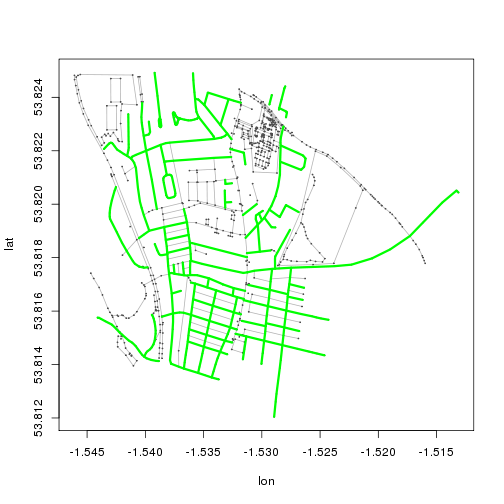
\includegraphics{figure/Residential_streets_in_Chapeltown.png}
\caption{Residential streets in Chapeltown}
\end{figure}

\section{Handling raw OSM data}

Although this section will be of most use for dealing with very large
files, a small example is used here to showcase the methods The file
\texttt{map.osm} downloaded directly from
\href{http://www.openstreetmap.org}{openstreetmap.org} is small,
allowing available on-line, from
\href{https://github.com/Robinlovelace/osm-tutorial/blob/master/data/map.osm?raw=true}{here}
(highlighting the advantages of open data for educational purposes -
there are few license restrictions).

The Java command line tool
\href{http://wiki.openstreetmap.org/wiki/Osmosis}{Osmosis} is used for
this purpose.

To show how Osmosis can subset raw OSM files, let us take a real world
example from the dataset we imported with the \texttt{osmar} package.
Imagine that we want to extract all osm data (nodes, ways and relations)
from the area in and around Potternewton Park. We could do this manually
by looking up the park on-line and selecting the associated elements in
QGIS. But imagine we want to do it from the command line (e.g.~for batch
processing). First we need a bounding box of all items containing the
text string ``Potternewton Park''. For this we use \texttt{osmar}:

\begin{Shaded}
\begin{Highlighting}[]
\NormalTok{potter <- }\KeywordTok{find}\NormalTok{(ctown, }\KeywordTok{way}\NormalTok{(}\KeywordTok{tags}\NormalTok{(}\KeywordTok{grepl}\NormalTok{(}\StringTok{"Potternewton Park"}\NormalTok{, ctown$ways$tags$v))))}
\NormalTok{potter <- }\KeywordTok{find_down}\NormalTok{(ctown, }\KeywordTok{way}\NormalTok{(potter))}
\NormalTok{potter <- }\KeywordTok{subset}\NormalTok{(ctown, }\DataTypeTok{ids =} \NormalTok{potter)}
\KeywordTok{plot_ways}\NormalTok{(potter)  }\CommentTok{# sanity check}
\end{Highlighting}
\end{Shaded}

\begin{figure}[htbp]
\centering

\includegraphics{figure/Line_data_of_Potternewton_park.png}
\caption{Line data of Potternewton park}
\end{figure}

\begin{Shaded}
\begin{Highlighting}[]
\NormalTok{potter.l <- }\KeywordTok{as_sp}\NormalTok{(potter, }\StringTok{"lines"}\NormalTok{)  }\CommentTok{# convert data to sp class}
\NormalTok{b <- }\KeywordTok{bbox}\NormalTok{(potter.l)  }\CommentTok{# save the bounding box}
\NormalTok{b[}\DecValTok{1}\NormalTok{, ] <- (b[}\DecValTok{1}\NormalTok{, ] - }\KeywordTok{mean}\NormalTok{(b[}\DecValTok{1}\NormalTok{, ])) * }\FloatTok{1.05} \NormalTok{+ }\KeywordTok{mean}\NormalTok{(b[}\DecValTok{1}\NormalTok{, ])}
\NormalTok{b[}\DecValTok{2}\NormalTok{, ] <- (b[}\DecValTok{2}\NormalTok{, ] - }\KeywordTok{mean}\NormalTok{(b[}\DecValTok{2}\NormalTok{, ])) * }\FloatTok{1.05} \NormalTok{+ }\KeywordTok{mean}\NormalTok{(b[}\DecValTok{2}\NormalTok{, ])}
\CommentTok{# scale longitude and latitude (increase bb by 5% for plot) replace 1.05}
\CommentTok{# with 1.xx for an xx% increase in the plot size}
\NormalTok{b}
\end{Highlighting}
\end{Shaded}

\begin{verbatim}
##      min    max
## x -1.529 -1.521
## y 53.817 53.822
\end{verbatim}

Now that we know the bounding box, we can transfer to using osmosis from
the command line. If the shell is open in the correct working directory
(e.g. ``osm-tutorial-master'', if downloaded from GitHub), the following
code will subset the data and output a new, smaller \texttt{.osm} file.

\begin{verbatim}
osmosis --read-xml data/map.osm --bounding-box top=53.822093 left=-1.528815 bottom=53.817486 right=-1.521155 --write-xml potter.osm
\end{verbatim}

To check whether or not this has worked, and demonstrate
\texttt{osmar}'s ability to read in \texttt{.osm} files, let us try to
load an plot the dataset just exported by osmosis.

\begin{Shaded}
\begin{Highlighting}[]
\NormalTok{src <- }\KeywordTok{osmsource_osmosis}\NormalTok{(}\DataTypeTok{file =} \StringTok{"data/potter.osm"}\NormalTok{)}
\NormalTok{bp <- }\KeywordTok{center_bbox}\NormalTok{(}\KeywordTok{mean}\NormalTok{(b[}\DecValTok{1}\NormalTok{, ]), }\KeywordTok{mean}\NormalTok{(b[}\DecValTok{2}\NormalTok{, ]), }\DecValTok{1000}\NormalTok{, }\DecValTok{1000}\NormalTok{)}
\NormalTok{potter <- }\KeywordTok{get_osm}\NormalTok{(bp, src)}
\end{Highlighting}
\end{Shaded}

\begin{verbatim}
## Warning: cannot open file '/tmp/Rtmpd8BxOn/file177f1a9cd644': No such file
## or directory
\end{verbatim}

\begin{verbatim}
## Error: cannot open the connection
\end{verbatim}

\begin{Shaded}
\begin{Highlighting}[]
\KeywordTok{plot}\NormalTok{(potter)}
\end{Highlighting}
\end{Shaded}

\begin{figure}[htbp]
\centering
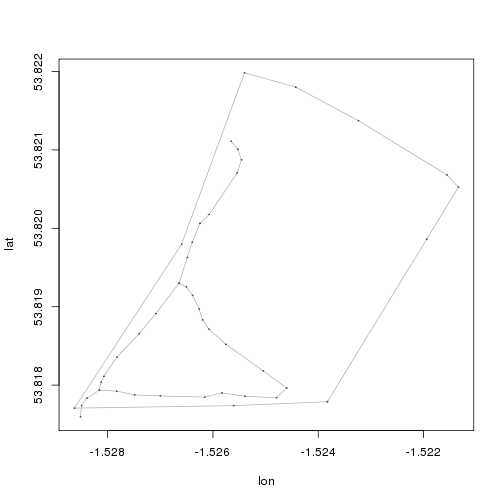
\includegraphics{figure/All_OSM_data_in_and_directly_surround_Potternewton_Park.png}
\caption{All OSM data in and directly surround
Potternewton Park}
\end{figure}

Local knowledge or a quick look on an online will confirm that this is
indeed Potternewton Park, with is rectangular tennis courts, play area
and skate park just west of its centre. The file \texttt{potter.osm} can
equally be loaded into QGIS or any other GIS. The point is to illustrate
how Osmosis works.

For further functionality, including clipping to polygons, extracting
files from enormous and compressed \texttt{planet.osm.bz2} files and
ways to extract only elements with certain attributes, please refer to
the \href{http://wiki.openstreetmap.org/wiki/Osmosis}{osmosis page of
the osm wiki}. The final section discusses (but does not implement) the
most advanced method of harnessing OSM data, via a PostGIS database.

\section{Creating a PostGIS database of OSM data}

There are a number of advantages of storing large datasets in a
database:

\begin{itemize}
\item
  The data can be accessed by a variety of 3rd party programs
\item
  Spatial queries can be made by a variety of clients accessing the db,
  widening the functionality
\item
  Huge datasets can be stored in a database, as it sits on the hard
  disk, only being transferred to RAM when a specific query is called
\end{itemize}

Because of the size and complexity of the planet-wide OSM database, it
must be stored in an spatial database to be used. For this use the
command line tool
\href{http://wiki.openstreetmap.org/wiki/Osm2pgsql}{osm2pgsql}. The
basics of installation and usage can be found online.

Using a spatial database, it does not take a very large leap to realise
that organisations can create a customised version of the OSM database
for their own purposes. For example, an organisation interested in store
location analysis could keep maintained a version of OSM with everything
with elements labelled as shops removed. Alternatively, an organisation
interested in woodlands could maintain an up-to-date version of OSM
woodlands. Both organisations could supplement these custom databases
with their own data, combining the best of crowd-sourced and centralised
data collection methods.

The \href{http://wiki.openstreetmap.org/wiki/Osm2pgsql}{OSM-GB} project,
hosted at the University of Nottingham does precisely this, with the aim
of quality-checking community contributed data. Here is not the place to
describe how to set-up a PostGIS database with OSM data, but is well
worth flagging as it has great potential, especially when combined with
rapidly evolving open source web mapping technologies such as
\href{http://geoserver.org/display/GEOS/Welcome}{GeoServer} (part of the
\href{http://geonode.org/}{GeoNode} stack),
\href{http://leafletjs.com/}{Leaflet} and
\href{https://www.djangoproject.com/}{GeoDjango}.

\section{Conclusion}

With the certainty of peak oil and possibility of effective climate
change regulations, transport will become increasing expensive in future
years. Thus, the tendency towards geographical homogenisation of
economic activity may go into reverse
(\href{http://books.google.co.uk/books?hl=en\&lr=\&id=mkV\_knlze0QC\&oi=fnd\&pg=PP2\&dq=ecotechnic+future\&ots=nATRuCVL31\&sig=bwafIZ7kfmZMK1EscQcKyIGeYsU\&redir\_esc=y\#v=onepage\&q=ecotechnic\%20future\&f=false}{Greer
2009};
\href{http://www.sciencedirect.com/science/article/pii/S0921800909003334}{Curtis
2009}). This is bad news for many, but it is good news for people with a
strong interest in regional diversity, local economies and geographic
diversity.

It is also potentially good news for geographers advocating for
location-specific solutions. With increased concern over the highly
centralised power structures of the internet following the revelations
leaked by Edward Snowdon about massive online spying and infringement of
digital privacy, there is a huge potential for community-based,
problem-specific solutions. It is with this wider context in mind that
this tutorial ends - think of the potential benefits if citizens were
encouraged to be both producers and consumers of the maps on which we
all now depend. Happy mapping!

\section{References}

Curtis, F. (2009). Peak globalization: Climate change, oil depletion and
global trade. Ecological Economics, 69(2), 427-434.

Eugster, M. J., \& Schlesinger, T. (2013). osmar: OpenStreetMap and R.
The R Journal, 5(1), 53-63.

Goodchild, M. F. (2007). Citizens as sensors: the world of volunteered
geography. GeoJournal, 69(4), 211--221.

Greer, J. M. (2009). The Ecotechnic Future: Envisioning a post-peak
world. New Society Publishers.

Haklay, M., \& Weber, P. (2008). Openstreetmap: User-generated street
maps. Pervasive Computing, IEEE, 7(4), 12-18.

Neis, P., Zielstra, D., \& Zipf, A. (2011). The street network evolution
of crowdsourced maps: OpenStreetMap in Germany 2007--2011. Future
Internet, 4(1), 1-21.

Salisbury, C. \& Jenkins, J. (2014). Mapping the Void. Broadcast on BBC
Radio 4, 11:00AM Mon, 27 Jan 2014. Available on I-Player until 11:32AM
Mon, 3 Feb 2014. Available on my
\href{https://dl.dropboxusercontent.com/u/15008199/egs2stay/Mapping\_the\_Void\_-\_Mapping\_the\_Void\_b03s6mf0\_default.m4a}{Dropbox
account} for forseable future.

Wroclawski, S. (2014). Why the world needs OpenStreetMap. The Guardian.
Tuesday 14 January 2014 11.52 GMT.

\begin{Shaded}
\begin{Highlighting}[]
\KeywordTok{source}\NormalTok{(}\StringTok{"md2pdf.R"}\NormalTok{)  }\CommentTok{# convert knitr document to LaTeX}
\end{Highlighting}
\end{Shaded}

\end{document}
